\documentclass{article}
\usepackage[a4paper, total={6in, 10in}]{geometry}
\usepackage{graphicx}

\title{Project 3 for PSYC 489}
\author{Bingjun Guo (bingjun3)}
\begin{document}
\maketitle
\section*{Part 1 Walsh Functions}
\subsection*{B.1}
Recordings on each run are in file Part1\_results.txt.\\
Mean hamming distance in each condition: [0.0, 1.65, 3.75, 4.2, 6.45, 7.95].\\
Mean time-to-settle in each condition: [0.0, 12.55, 19.75, 23.1, 24.65, 25.3].\\
The network hasn't failed to settle in each probability condition.
\subsection*{B.2}
Detailed energy recordings are in Part1\_energy.txt. A plot of energy changes on each run is provided below, and we can tell from the plot that energy isn't always decreasing. It increases occasionally. Detailed energy recording is provided in file Part1\_energy.txt.
\begin{figure}[h]
    \centering
    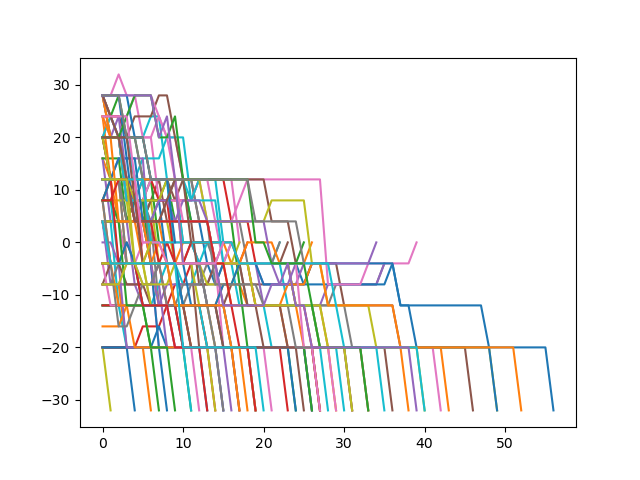
\includegraphics[width=8cm]{Part1energy}
    \caption{Energy on each run in part 1}
\end{figure}
\newpage

\section*{Part 2 Random Patterns}
Recordings on each run are in file Part2\_results.txt. Interpretation: It will be harder for the model to settle, that is, both time-to-settle and hamming distances will be larger.\\
Mean hamming distance in each condition: [1.67, 3.07, 4.53, 5.6, 6.47, 6.73].\\
Mean time-to-settle in each condition: [12.2, 19.2, 29.33, 29.47, 31.6, 34.6].\\
The network hasn't failed to settle in each probability condition. Detailed energy recording is in file Part2\_energy.txt.\\
\begin{figure}[h]
    \centering
    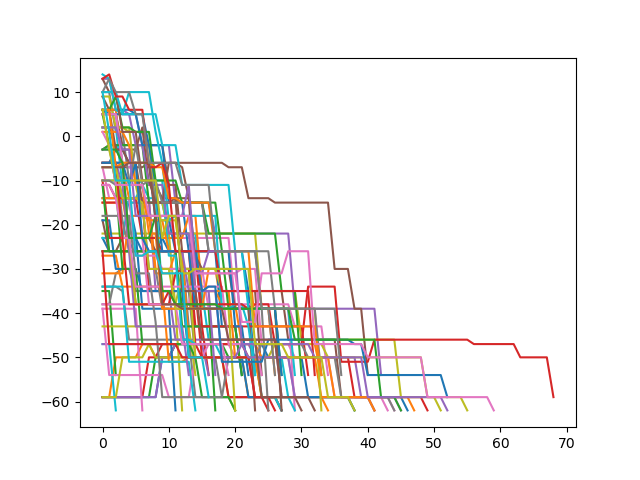
\includegraphics[width=8cm]{Part2energy}
    \caption{Energy on each run in part 2}
\end{figure}\\
It can be observed that mean hamming distances between and time-to-settle are indeed larger, even though the number of training and testing patterns is less. What's more, when the probability is 0, that is, the starting state is exactly the same as a training pattern, the model can fail to settle. For random patterns, the learning capacity of a Hopfield Network is given as:
\[C = \frac{n}{2\log_2n}\]
which equals to $\frac{16}{2\cdot4} = 2$ in our case, thus 3 random patterns exceeds this limit. For Walsh function pattern, the limit can rise higher.\\
In the following runs on two extra patterns, mean hamming distances are 6.6, 5.2 and mean time-to-settle are 37.0, 21.0. Meanwhile, when the probability is 0.2, previous mean values are 4.53 and 29.33. It can be told that hamming distances are larger for the latter two patterns, and time-to-settle are occasionally larger. In Further experiments, it can be observed that they are mostly larger in last two patterns.
The reason for this can be due to the limitation of the model learning capacity, as the model is trained on more pattern, it's less likely to remember the training patterns.
\newpage

\section*{Part 3 Systematically Related Patterns}
Detailed recordings are in Part3\_result.txt and Part3\_energy.txt.\\
Mean hamming distance for each pattern: [0.167, 0.167, 0.33, 0.167, 0, 0.167].\\
Mean time-to-settle for each pattern: [2.53, 0.833, 1.0, 3.4, 0.0, 3.1].\\
Again, it doesn't appear that the network ever fails to settle. Meanwhile, for all runs, they settle to the base pattern.
It can because that since all the training patterns are related, the network successfully remember the way that they are in common, that is, the prior distribution of them.
For the corresponding psychological phenonmenon, I'm not majoring in Psychology, and ChatGPT tells me that it's referred as ``pareidolia'' or ``apophenia'', which point to human's tendency to ``perceive patterns where none exist, or to find meaning in random or unrelated data''.
Energy states are provided below:
\begin{figure}[h]
    \centering
    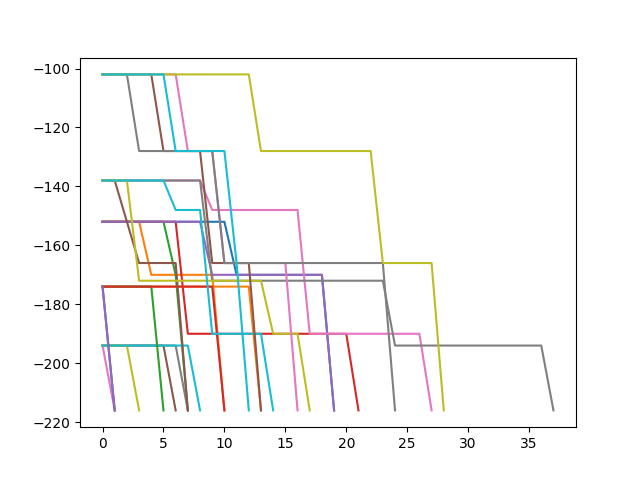
\includegraphics[width=8cm]{Part3energy}
    \caption{Energy on each run in part 3}
\end{figure}\\

\section*{Part 4 Asynchronous Updating}
In this part I select walsh functions in part 1 as the training patterns for 5 times, updating 1 (asynchronously), 2, 4, 8, 16 (synchronously) units at most in each iteration.
It turns out that as the maximum number of units that can be updated in each iteration increases, the chance for the network to fail to settle increases.
At the same time, the higher the noises are, the higher such chance would be.
Still, recordings are in file Part4\_results.txt. ``None'' means that the network fails to settle within 1234 iterations. An example set of energy states for fully synchronously updating is also recorded, provided in Part4\_energy.txt. It's also plotted as below:
\begin{figure}[h]
    \centering
    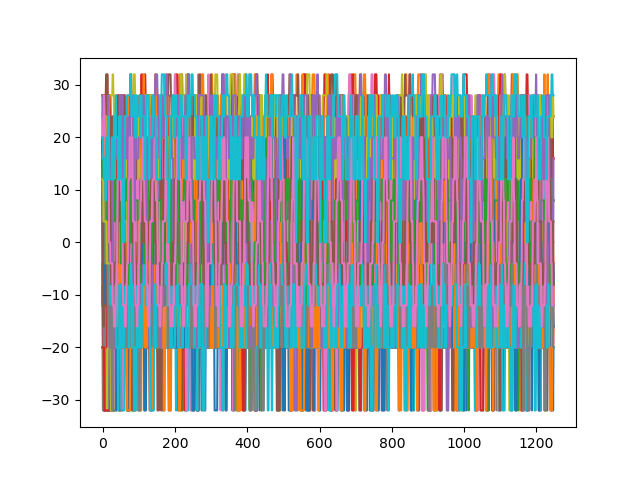
\includegraphics[width=8cm]{Part4energy}
    \caption{Energy on each run when updating synchronously}
\end{figure}
\end{document}
